\chapter{\sffamily Multi-stage pipelines}

{\bfseries\sffamily Concept.} Building a toy model simulation of a rugby match whose outcome can be manipulated through correctly-timed player substitutions and game management decisions. The state manipulation framework we have built around the stochadex can meet these requirements, and a dashboard can be created for user interaction. All this combines together to make a simple dashboard game, which we call: `trywizard'. For the mathematically-inclined, this chapter will motivate the construction of a specific modeling framework for rugby match simulation. For the programmers, the public Git repository for the code described in this chapter can be found here: \href{https://github.com/umbralcalc/trywizard}{https://github.com/umbralcalc/trywizard}.

\begin{figure}[h]
\centering
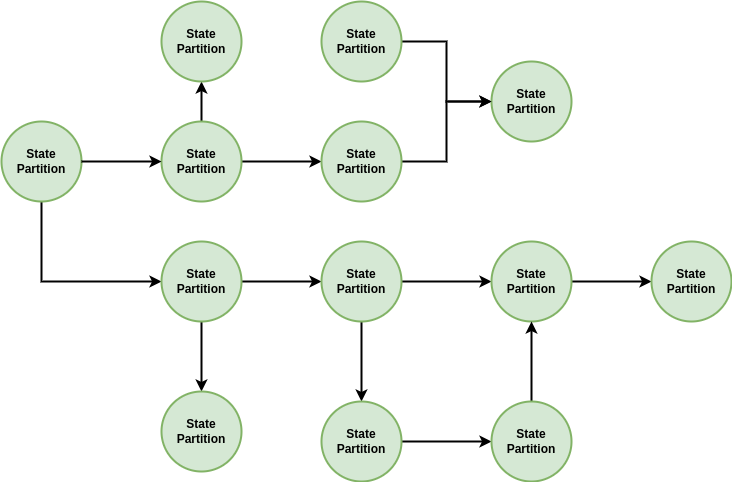
\includegraphics[width=12cm]{images/chapter-9-state-partition-graph.drawio.png}
\caption{State partition graph topology for multi-stage pipeline archetypes.}
\label{fig:state-partition-graph-multi-stage-pipelines}
\end{figure}
